El tiempo que tarda una onda en completar un ciclo de oscilación. Se representa con la letra $T$ mayúscula. Se mide en segundos $s$.

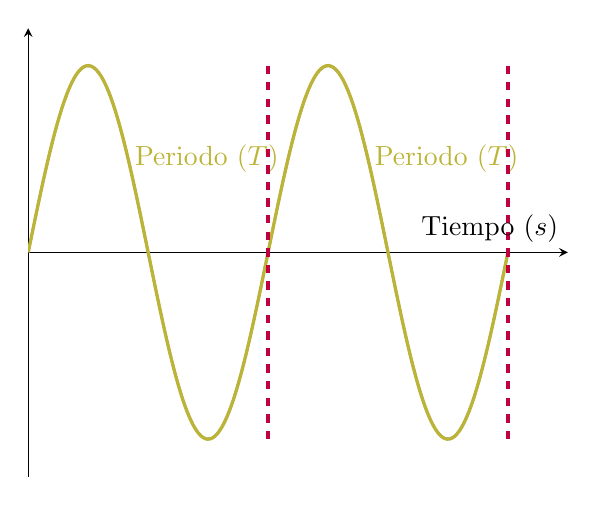
\begin{tikzpicture}
  \begin{axis}[
    xmin=0,xmax=4.5*pi,
    ymin=-1.2,ymax=1.2,
    axis lines=middle,
    xtick={0},
    ytick={0},
    xlabel=Tiempo ($s$)
    ]

    % Funcion senoidal
    \addplot[color=blue,samples=100,domain=0:4*pi,thick]{sin(deg(x))};

    % Periodo 1
    \addplot[color=yellow!70!black,samples=100,domain=2*pi:4*pi,very thick]{sin(deg(x))};
    \node[yellow!70!black,right,very thick] at (axis cs:2.8*pi,0.5) {Periodo ($T$)};

    % Periodo 2
    \addplot[color=yellow!70!black,samples=100,domain=0:2*pi,very thick]{sin(deg(x))};
    \node[yellow!70!black,right,very thick] at (axis cs:0.8*pi,0.5) {Periodo ($T$)};

    % Lineas verticales
    \draw[purple,dashed,very thick] (axis cs:2*pi,1) -- (axis cs:2*pi,-1);
    \draw[purple,dashed,very thick] (axis cs:4*pi,1) -- (axis cs:4*pi,-1);
  \end{axis}
\end{tikzpicture}

Se puede calcular como el tiempo transcurrido en segundos entre la cantidad de ciclos completos.

\[
  T=\dfrac{\text{tiempo} (s)}{\text{número de ciclos}}
\]
